%\setcounter{chapter}{2}

\chapter{LHC and the CMS experiment}
\label{ch:cms}
CERN accelerator complex is a sequence of machines that produces and accelerates "bunches" of $10^{11}$ protons to nearly the speed of light. In the Large Hadron Collider (LHC) the bunches collide at specific interaction points (IP), where the four main experiments are located: ALICE, ATLAS, CMS, and LHCb. We will start this section with the discussion of the LHC machine and then describe the CMS detector. 

\section{The Large Hadron Collider}\label{sec:cms_intro}
\subsection{The history of the LHC}

The story of the LHC begins in 1977, when the CERN director general Sir John Adams suggested that the tunnel of the Large Electron-Positron Collider (LEP) can be reused to accommodate the future hadron collider of more than 3 TeV energies \ref{Sadenius}. At the 1984 ECFA-CERN workshop on a "Large Hadron Collider in the LEP Tunnel" \ref{LHC1984}, the physics goals of the LHC were stated: confirmation of the BEH mechanism, search for the Higgs Boson, and exploration of the origin of masses of W and Z bosons. The parameters of the proposed LHC were very ambitious: the centre-of-mass (COM) collision energy of 10 to 20 TeV, and a target instantaneous luminosity of 10$^{33-34}\frac{1}{cm^{2}s}$. 

Large Hadron Collider (LHC) is the most powerful particle accelerator that has ever been built. It is located at the border of France and Switzerland at a depth from 50 to 175 m underground. LHC ring is 26.7 km in circumference and it is the final stage in a sequence of accelerators. 


\begin{figure}[H]
  \centering
%  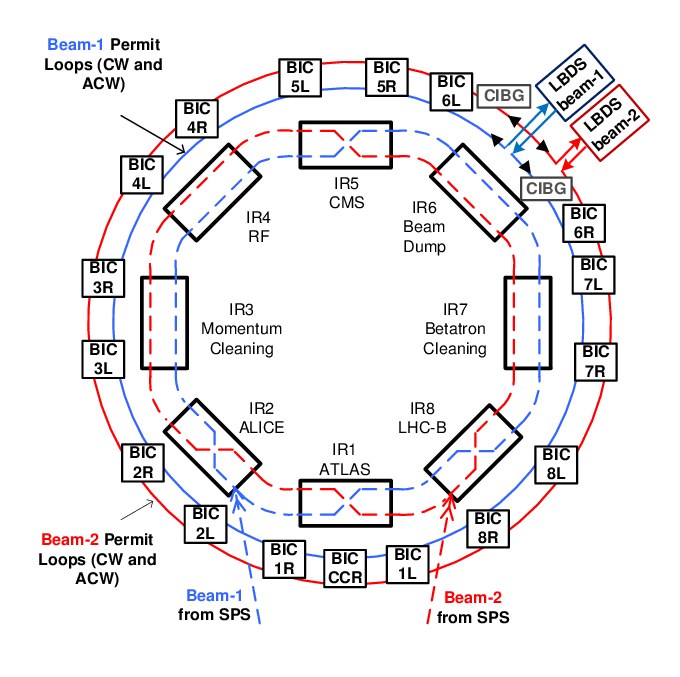
\includegraphics[width=0.75\textwidth]{LHC-beam-permit-loops}\\
  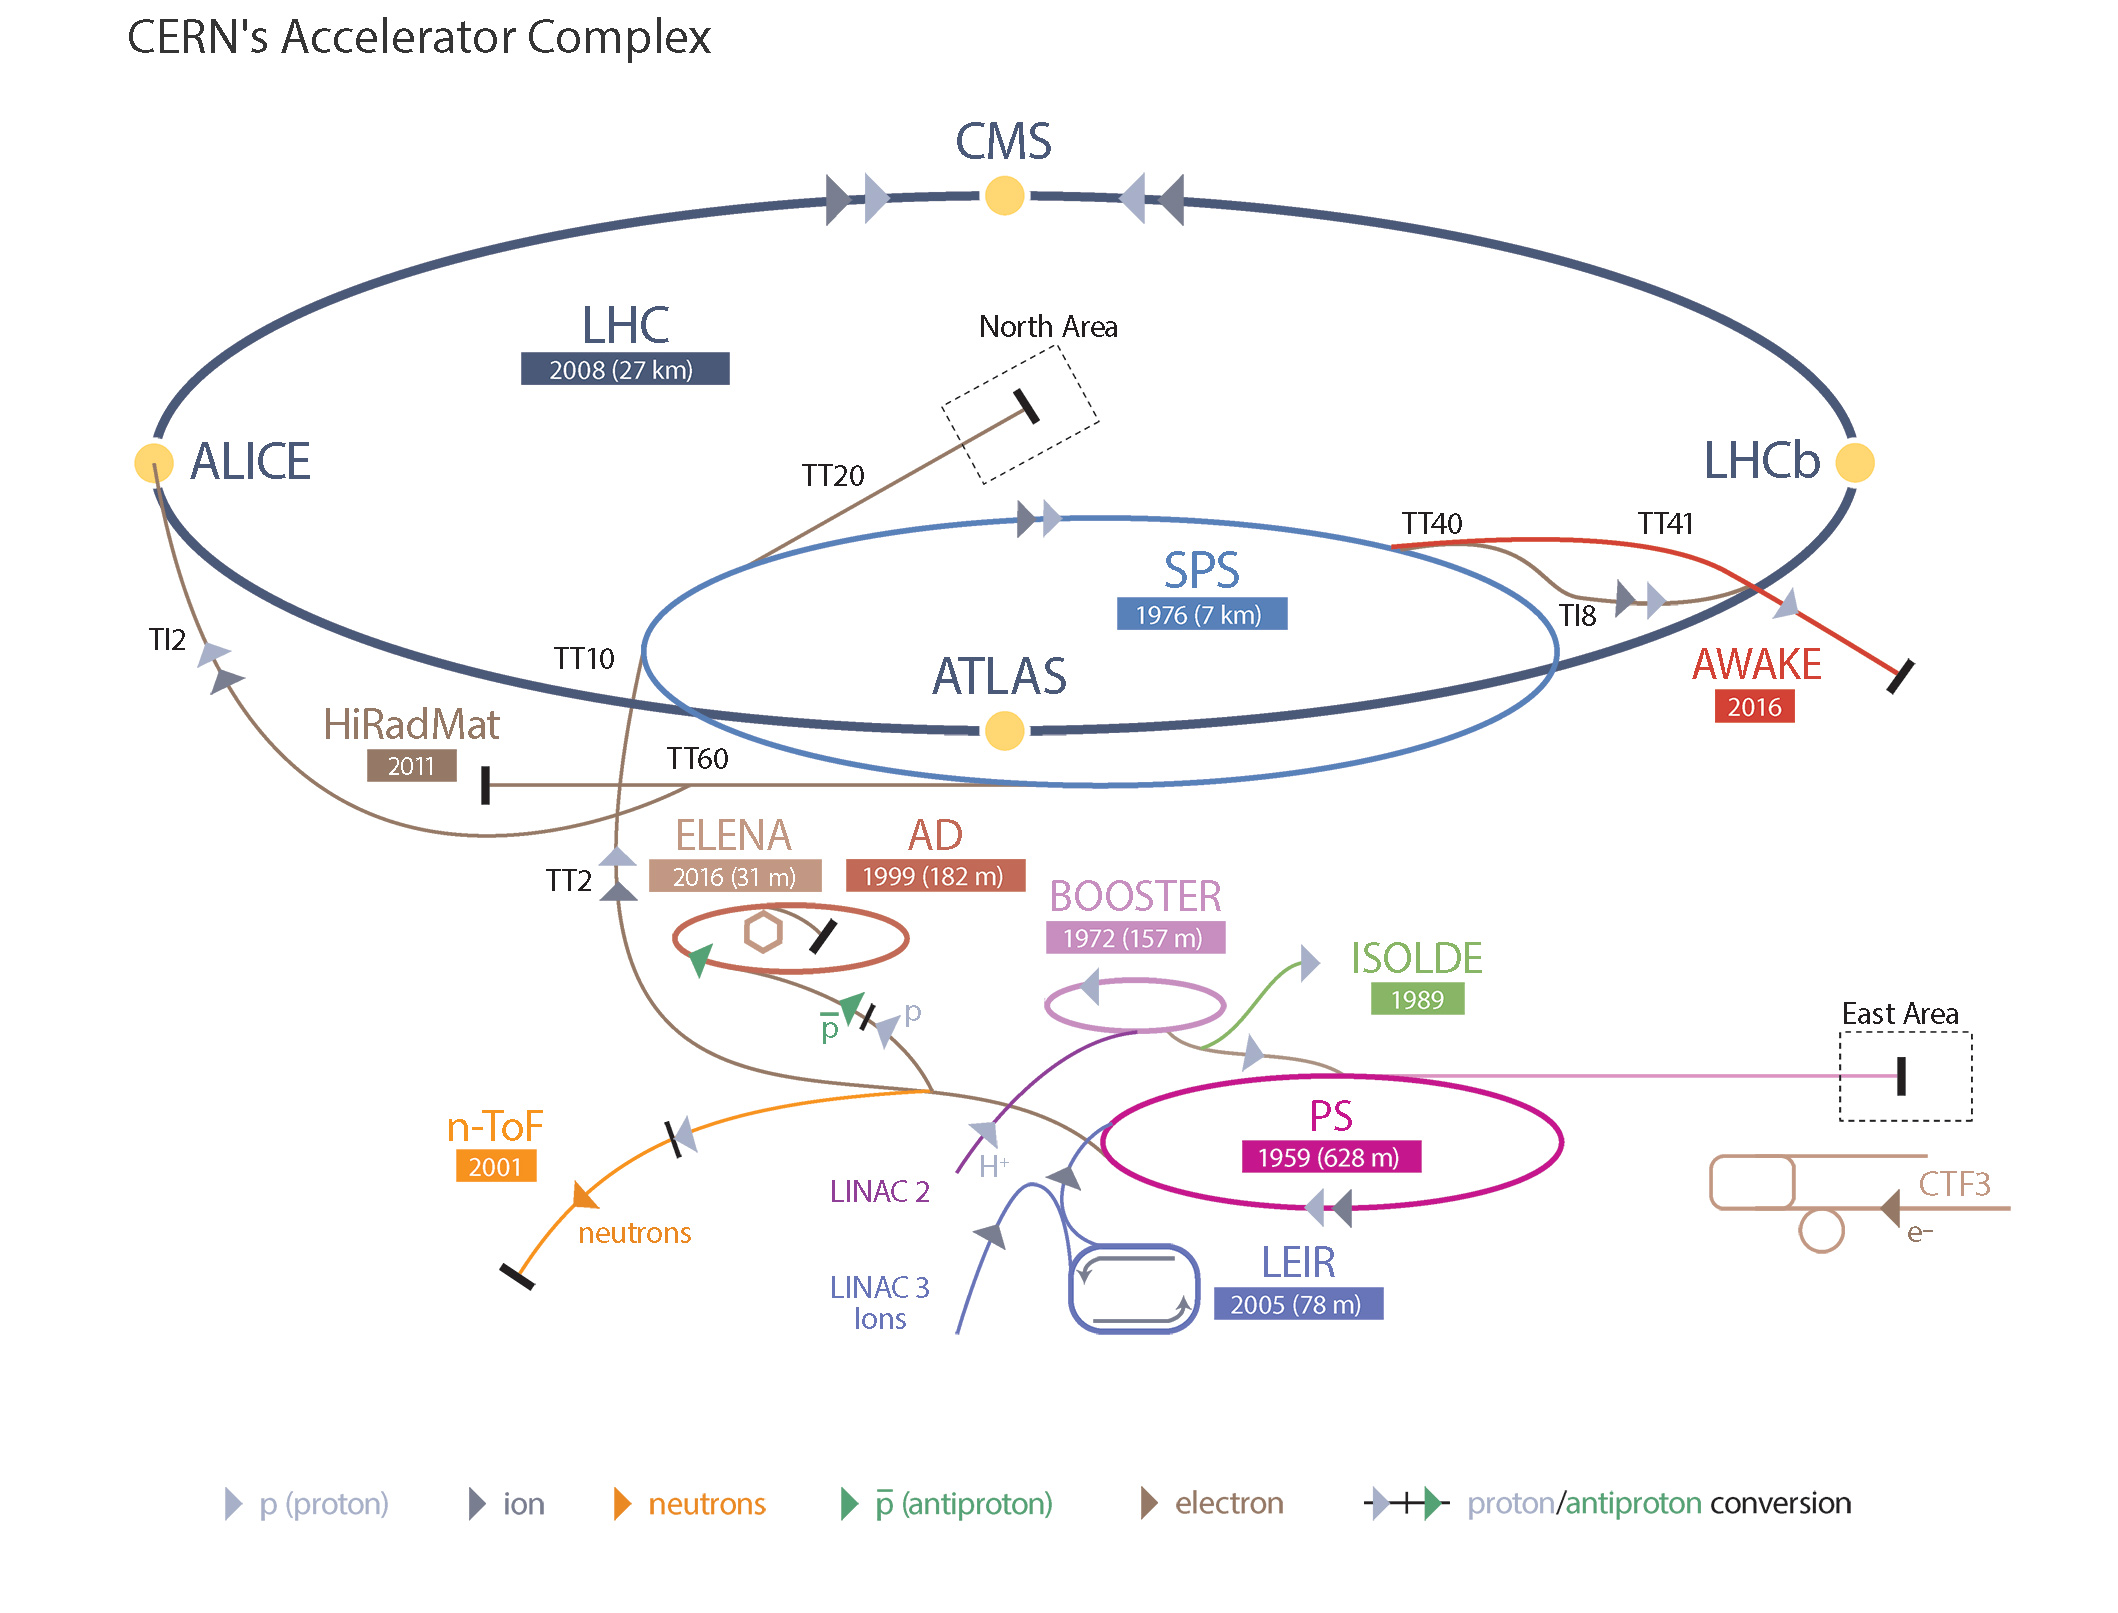
\includegraphics[width=0.75\textwidth]{LHC_default.jpg}
  \caption {Schematic layout of the LHC.}
  \label{lhcmap}
\end{figure}


It is a complex process to start proton-proton collision in the LHC at 13 TeV and, therefore, the process consists of several stages (see Fig. \ref{lhcmap}). Everything begins with the bottle of hydrogen. The hydrogen atoms from the bottle are fed into the source chamber of the Linear Accelerator (Linac). In the chamber the hydrogen is heated up to the plasma state until electrons are stripped off of the hydrogen atoms. Then electrons are removed and remaining protons are directed to the first acceleration stage which increases the energy of protons to 50 MeV. After Linac, the beam of protons is injected into the Proton Synchrotron Booster (PSB). PSB contains four rings each accelerating a bunch of protons (a moving collection of protons of a narrow length) to 1.4 GeV. The third stage is the Proton Synchrotron (PS), which splits the incoming beam into 72 bunches separated by 7.5 m. The energy of the protons is increased to 25 GeV. After that, the protons are sent to the Super Proton Synchrotron (SPS), where they are accelerated to 450 GeV. SPS then fills the LHC ring with two beams each consisting of 2808 bunches of protons with nearly $10^{11}$ protons in total. It takes SPS about $O(10)$ minutes to fill each LHC ring with bunches. In the LHC two beams are circulating in opposite directions in two separate beam pipes. During standard data taking beams circulate for $O(10)$ hours.  


\subsection{LHC operations}

The first LHC budget plan was finalised in 1996 and the final cost was approved just a few years later. The first proton beam entered the LHC ring in 2008. However, an incident intervened the LHC plans. It was caused by the mechanical damage of the tunnel equipment due to the release of the helium. Thus, the real data taking period (called LHC Run-1) had started only in 2010 and lasted for two years with 7-8 TeV COM energies. The recorded dataset contained enough Higgs bosons to claim a discovery of this rarely produced particle. After this achievement, the LHC was closed for the first long shutdown (LS1) that happened in 2012. During this time necessary upgrades of the main detectors and the LHC were performed. This was an unavoidable and essential step to prepare the LHC for more challenging environment of COM energies increased to 13 TeV. 


If we denote the area of 10$^{-28}$ $m^2$ as barn (b), then in terms of these new units the LHC can theoretically produce $80-120/fb$ of data a year. In practice numbers were lower, because LHC operated at the revolution frequency below the nominal, used fewer proton bunches in the beam, etc.  All this resulted in lower than expected instantaneous luminosity, which is a very important term in collider physics and will be explained in the next section.

The LHC Run-2 has started in 2015 and the CMS collected 4.2 $fb^{-1}$ of data that year. Over the course of the 2016 data taking, an integrated luminosity of 35.9 $fb^{-1}$ was recorded. This luminosity is the amount of data that has been collected by the CMS detector and later approved by the CMS physics coordination for the use in the physics analyses. The data set of proton-proton collisions collected in 2016 at 13 TeV COM energy is used in this thesis to analyse double Higgs boson decays. Together with the 2017 and 2018 data taking, almost 150 $fb^{-1}$ have been delivered and recorded by the CMS detector during the whole Run-2 period of four years. 

At the moment of writing this thesis, the LHC has entered the LS2. The next data taking will resume in 2020 and proton-proton collisions will continue for three years with the expected delivered integrated luminosity equal to nearly 300 $fb^{-1}$. This will conclude the LHC Phase-1 programme. 

The new upgraded LHC, the High-Luminosity LHC (LHC) or the Phase-2, will start operations in 2026 and run until 2035. The COM energy will be increased to 14 TeV and one expects to record an unprecedented dataset of 3000 $fb^{-1}$. 

\subsection{Luminocity}

%The quantity that measures the ability of a particle accelerator to produce the required number of interactions is called the luminosity and it is the proportionality factor between the number of events produced per second dR/dt and the cross section of the process \cite{Herr:941318}



The instantaneous luminosity is the coefficient which relates the cross section $\sigma$ of the process to the number of events $N_{events}$ produced during the interaction: $N_{events} = \mathcal{L}  \sigma$. Luminosity is the parameter controlled by the machine and can be written as:

$ \mathcal{L} =\frac{N^2 n_b f_{rev}}{4\pi \sigma_x \sigma_y}$

\noindent where $N_b$ is the number of particle in the colliding bunch, $n_b$ is the number of colliding bunches in the beam, $f_{rev}$ is the revolution frequency of the beam, $\sigma_x$ and $\sigma_y$ are the standard deviations of the beam density profile (BDP) in the transverse plane, where it is assumed that the BDP of both beams can be described by a Gaussian distribution.


To maximise the amount of collected data, the luminosity parameter should be as high as possible. It is worth noting that the luminosity is not constant and decays with time due to the degradation of the initial circulating beams. Theoretical decay time (the time to reach $1/e$ level) is approximately 29 h. In practice, taking into account the decrease of protons in the bunch due to collisions, contributions from the intrabeam scattering, scattering on the residual gas, etc., the real luminosity lifetime is about 15 h. 

A useful variation of the luminosity parameter is a total integrated luminosity. This is the number normally quoted for the dataset collected over the period T:

$L = \int_{0}^{T} \mathcal{L}  dt$.

In collider physics the "beam dump" is a process of burning off exhausted low luminosity beams by intentionally directing them towards the target made of concrete and steel. The time from the start of the collisions to the beam dump is usually called the "run".

We can calculate the amount of data delivered by the LHC during a single run period $O(10)$ h. Performing the integration, we obtain: 

 $L = \mathcal{L}_0 \tau_\mathcal{L}  \left[  1- e^{\frac{-\tau_{run}}{\tau_\mathcal{L} }}  \right]$, 

\noindent where $\mathcal{L}_0$ is the initial peak instantaneous luminosity at the start of the run, $\tau_{run}$ is the total duration of a run, and $\tau_\mathcal{L}$ is the luminosity lifetime. The optimum run time is 12 hours. During the runs, the LHC centre needs to dump the old beams, fill the rings with the new beams, and increase ("ramp") the energy of new beams to 13 TeV. After that a new run can be started. This restarting process normally takes two to six hours.



\subsection{LHC infrastructure}

The equipment of the LHC tunnel serves several purposes with the main objective to keep the colliding beams on the circular orbit. This requires a complex synchronised work of bending dipole magnets, cooling systems, accelerating radio frequency cavities, and vacuum insulation systems.

\subsubsection{Magnets}\label{sec:magnets}

Most of the LHC circumference is used by 1232 superconducting magnets placed evenly around the tunnel to approximate the circular orbit. These are dipole magnets (see Fig. \ref{dipoles_coils}) that bend the beam and keep it on the circular orbit, that is why they are commonly called "Main Bends" (MB). The proven technology existed since Tevatron and relied on NbTi superconductors. This technology also satisfied the LHC cost and performance requirements, thus, it was decided to reuse the same choice of the alloy for the LHC superconducting dipole magnets that steer the proton beams. 

The dipoles need to produce the magnetic field of 8.3T. % and it requires a current of about 11kA. 
Each dipole is 16.5 $m$ (with ancillaries) long and 570 $mm$ in diameter and is placed inside of the dipole cryostat which is called the "Helium bath". 

This cryostat is a long cylindrical tube 914 $mm$ in diameter made of low-carbon steel, where the dipole mass is cooled down to 1.9 $K$. Even though the inner structure of such cryostat is very complex and includes two beam pipes, two sets of coils for two beam pipes, vacuum pipes etc., one normally calls this compound object simply a dipole magnet. The name "dipole" is reserved for MBs since for each beam pipe the magnet consist of two "poles" that provide a vertical magnetic field similarly to a simple dipole system of magnets. 

\begin{figure}[H]
\centering
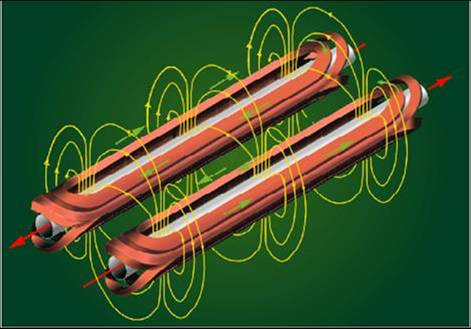
\includegraphics[width=0.65\textwidth]{dipole_1.jpg}\\
\vspace{0.5cm}
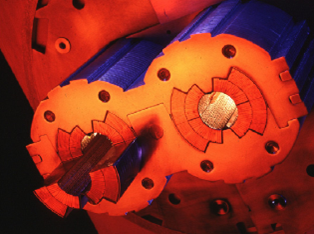
\includegraphics[width=0.65\textwidth]{dipole_2.png}
\caption[LHC dipoles]{LHC dipole magnets. Top: two dipole coils and magnetic field lines. Bottom: two beam pipes with the coils inside of the dipole magnet. }
\label{dipoles_coils}
\end{figure}



A  dipole magnet  must  be  curved to help a chain of dipoles complete 360 degrees. The curvature is 5.1 $mrad$ per dipole, which is equivalent to a  sagitta of  about  9 mm, corresponding to a radius of curvature of 2812.36 m.


The other important set of magnets is quadrupoles. They are used to ensure the proper beam dynamics. In total 392 quadrupole magnets ranging from 5 to 7 metres in length are used to squeeze the beam in transverse direction and to keep it narrow during the run duration. Additional special quadrupole magnets (SQM) are installed right before the IPs to focus the beams even more. That increases the density of protons in the beam and guarantees the maximum luminosity. In addition, SQMs help to decrease the chance of the parasitic collisions when bunches from the same beam or bunches outside of the IP centre interact (see Fig. \ref{quadrupoles}). To further correct the beam path (orbit), about 5000 higher order correcting magnets are used, which are evenly spaced around the circular trajectory of the LHC. 


\begin{figure}[H]
\centering
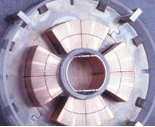
\includegraphics[width=0.4\textwidth]{quad_2.png}
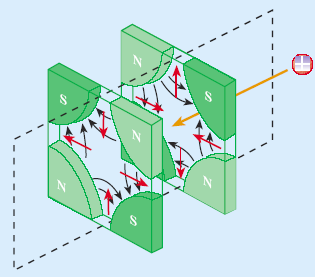
\includegraphics[width=0.37\textwidth]{quad_1.png}\\
\vspace{0.5cm}
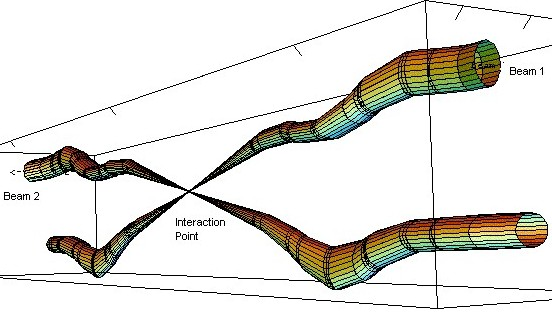
\includegraphics[width=0.7\textwidth]{quad_3.jpg}
\caption[LHC quadrupoles]{LHC quadrupoles. Top left: the coil of the quadrupole magnet. Top right: schematic view of the magnetic fields in the quadrupole. Bottom: two beams and the IP.}
\label{quadrupoles}
\end{figure}


To power the LHC, 1612 electrical circuits are used. Mostly these circuits are needed to power the dipole and quadrupole magnets, which is done in eight evenly spaced location of the LHC. A total of 3286 current leads are needed to connect all the circuits and power cables. More than a thousand of the leads operate between 600 A and 13 kA (see Fig. \ref{13kA_lead}). The other leads work in the range 60 to 120 A. 

\begin{figure}[H]
  \centering
  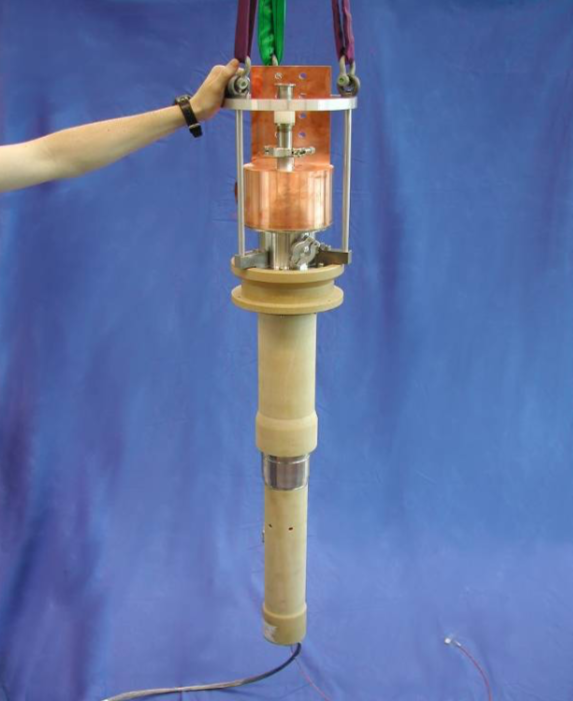
\includegraphics[width=0.5\textwidth]{13kA_lead}
  \caption{13 kA high-temperature superconducting current lead.}\label{13kA_lead}
\end{figure}



\subsubsection{Cooling System}\label{sec:cryogenic}

To ensure that dipoles are in the superconducting state, they have to be cooled to 1.9 K using superfluid helium-4. 

The cooling (cryogen) system is needed to keep superconducting LHC magnets at the appropriate temperature. The choice of the cooling gas depends on the magnet type and location. This dictates the required range of temperatures, which differs from system to system by 75 K. The cryogen system uses layered design with the temperature becoming progressively colder going from outside the dipoles closer to the beam pipe. 

The "coldest" part of the cryogen system is designed for the inner part of the dipoles. This system (see Fig. \ref{cryo_T_scale}) must cool down 37 Mkg of the LHC magnets within 15 days to the required temperatures, which is done through the system of pipes that transport the flow of the superfluid helium. The cryogen system must also be able to deal with the fast increases of the pressure flow and flow surges, as it is crucial for the LHC operation to keep dipoles constantly cooled and at the superconducting state.


The LHC tunnel is inclined in the horizontal plane by 1.41$^\circ$. This translates to 120 m difference in the vertical location of two diametrically opposite points of the tunnel with respect to the surface level and results in the additional hydrostatic pressure that can affect the flow of helium. This has been an important concern during the design of the cryogen system.


Since the cost to cool the LHC parts to 1.8-1.9 K temperatures is high, several temperature levels are employed (see Fig. \ref{cryo_T_scale}):
 
\begin{itemize}
\item 50 to 75 K for the thermal shielding used in the dipoles,
\item 20 to 300 K for upper ("warm") sections of the high-temperature superconducting current leads,
\item 4.6 to 20 K for lower temperature interception,
\item 4.5 K for radio frequency cavities and lower ("cold") sections of the high-temperature superconducting current leads,
\item 4 K for the transportation system that directs the 1.8 K helium to dipoles,
\item 1.9 K for helium in the superfluid state to cool magnet masses.
\end{itemize}

\begin{figure}[H]
  \centering
  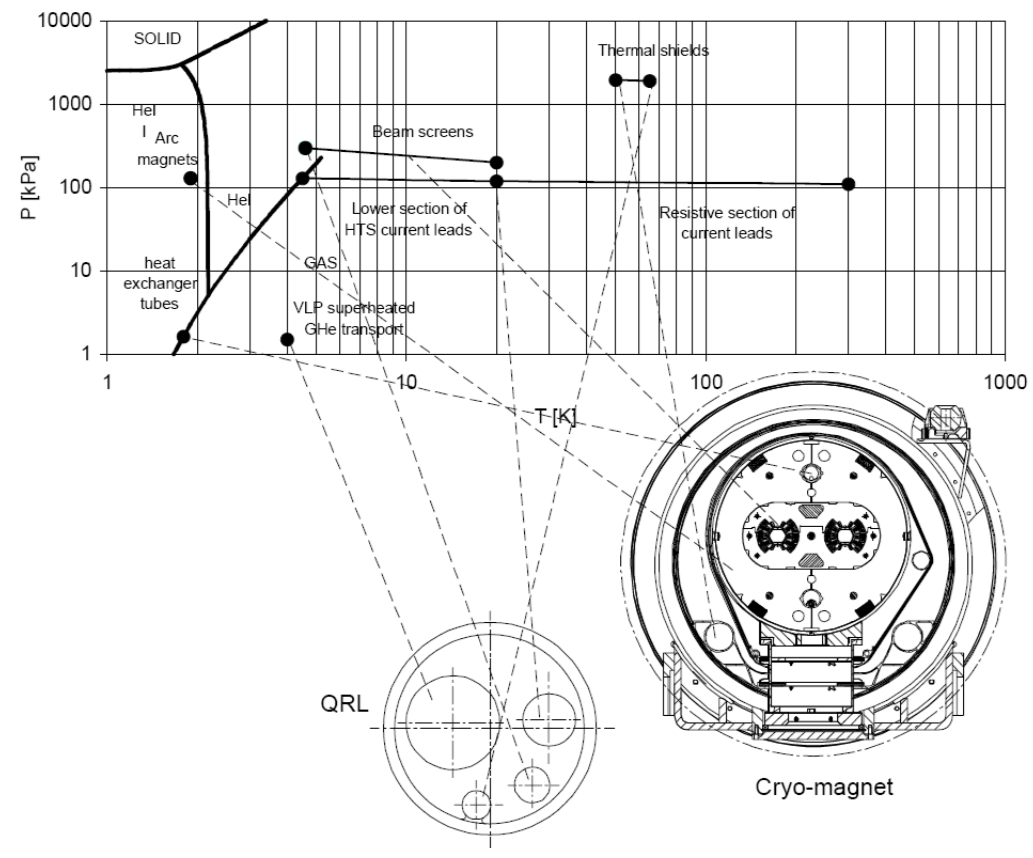
\includegraphics[width=0.7\textwidth]{cryo_T_scale}
  \caption{LHC cryogenic states and the temperature scale.}\label{cryo_T_scale}
  \label{cryo_T_scale}
\end{figure}




\subsubsection{Radio Frequency Cavities}\label{sec:rf}


Proton bunches need to be ramped to 7.5 TeV energies. To achieve this 13 TeV COM energy, eight superconducting radio-frequency cavities (RFC) are used per beam. They are located in front of the IPs of four experiments. Electromagnetic waves of 400 MHz with a peak field strength of 5.5 MV/m adjust the speed of protons in bunches. Each RFC (see Fig. \ref{lhc_rfc}) increases the energy of protons by 60 keV per revolution and it takes $O(20)$ minutes to reach 6.5 TeV beam energy. The RFC frequencies are increased gradually by 1 kHz to match the speed up of protons in the bunch as they gain more energy. When the ramp is completed, the RFCs are used to compensate for small energy losses due to the synchrotron radiation (7 keV per revolution). 




\begin{figure}[H]
\centering
%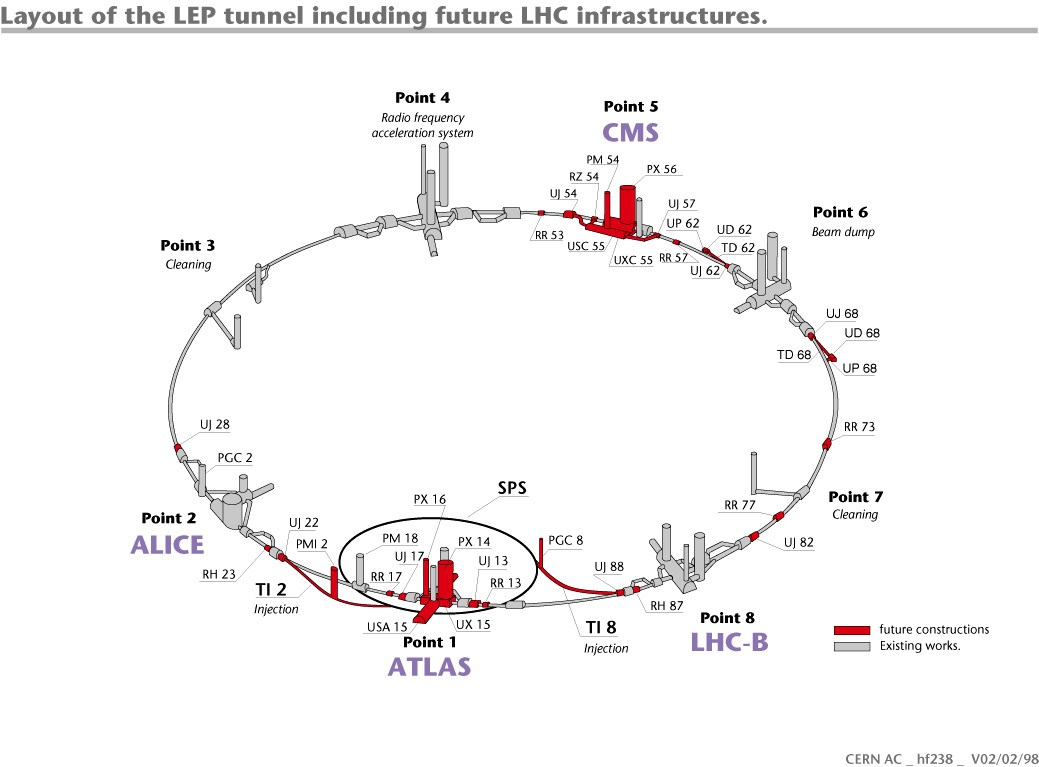
\includegraphics[scale=0.6]{lep}
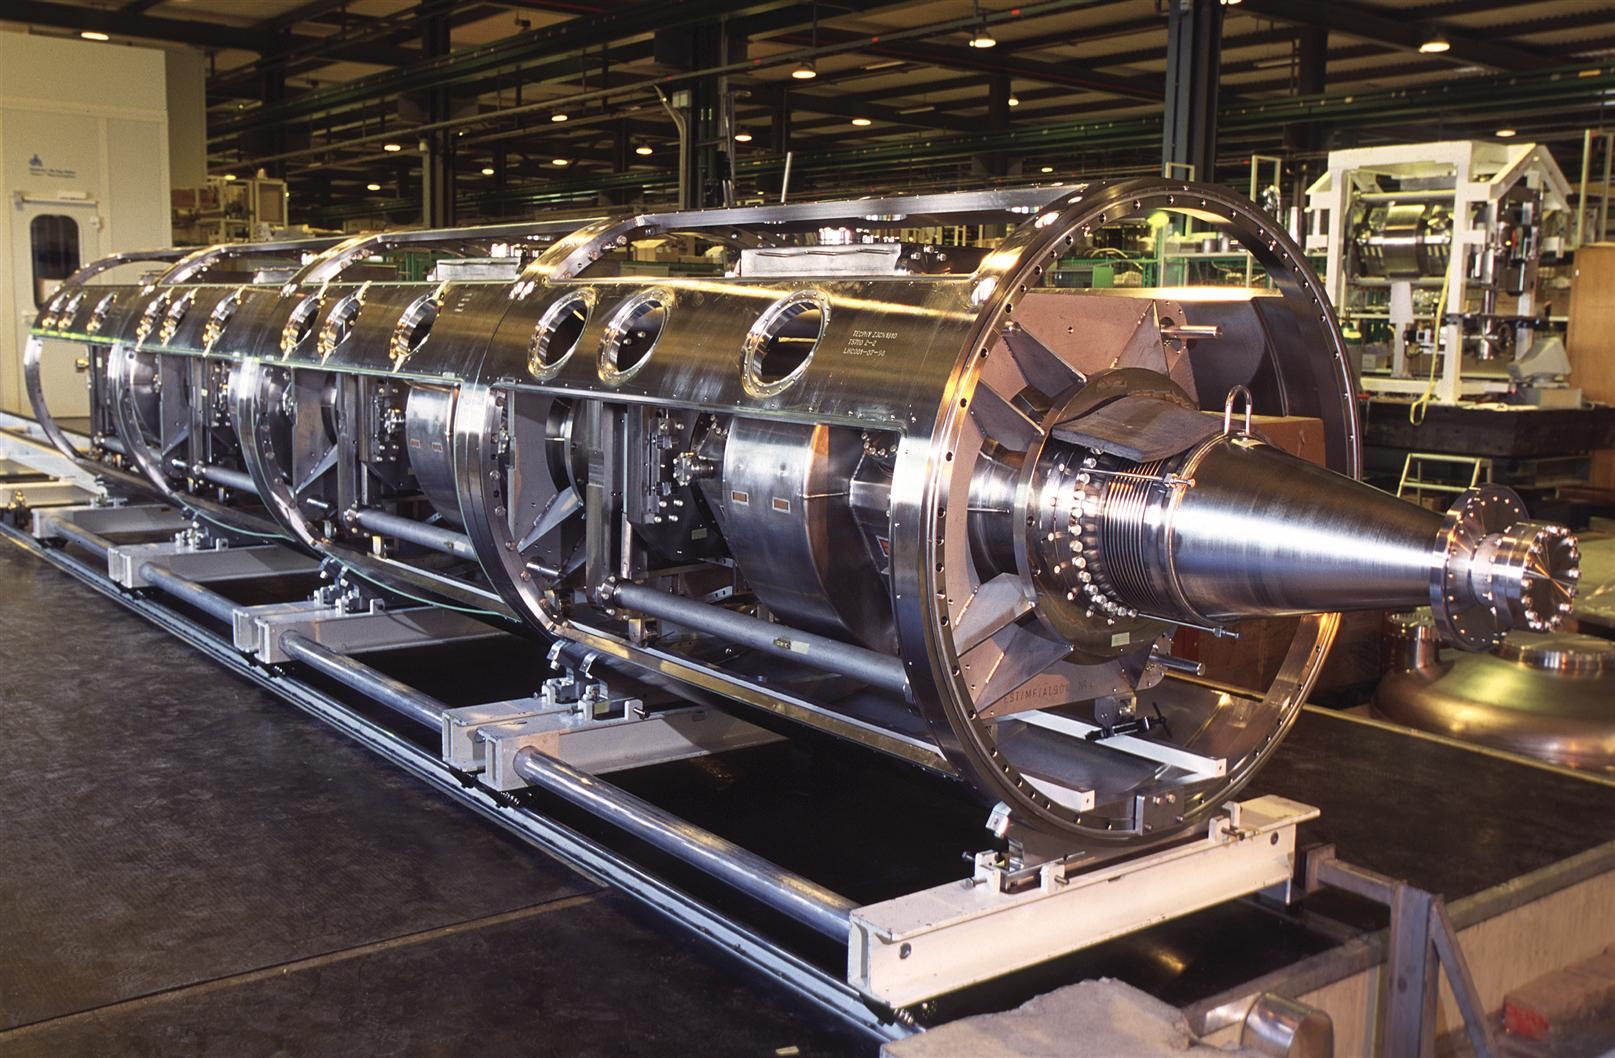
\includegraphics[width=7cm,height=4.2cm]{lhc_rfc}
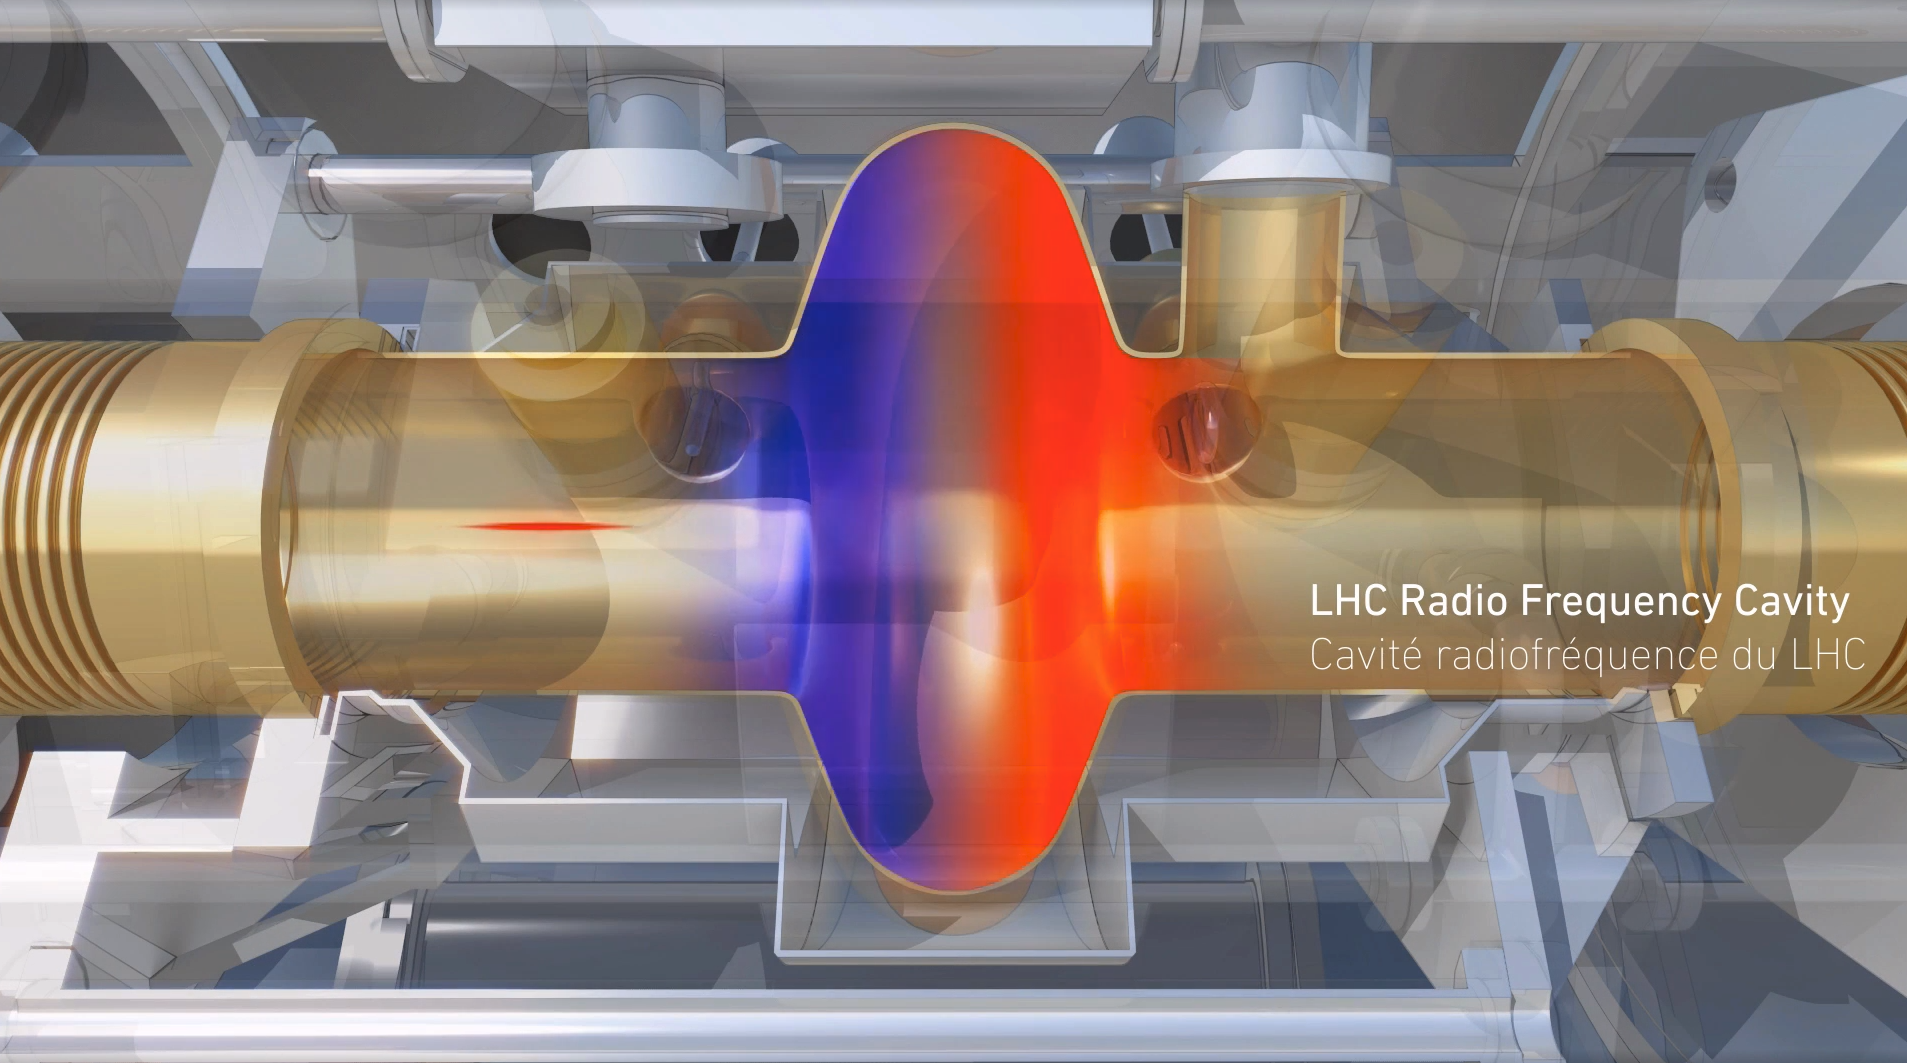
\includegraphics[scale=0.15]{rfc_lhc}
\caption[RF cavities module.]{LHC RF cavities. Left: a cryomodule with four RF cavities. Right: a schematic drawing of a single RF cavity. The colour field is used to denote Positive (red) and Negative (blue) polarities. A narrow beam traversing the cavity is shown in red. }
\label{lhc_rfc}
\end{figure}




\subsubsection{Vacuum System}\label{sec:vacuum}



The work of the LHC depends on three vacuum systems \cite{LHC_vacuum}. Without them, dipoles will not be at the superfluid state, the beams will not be able to circulate, and no stable collisions would be taken. With a total of 104 kilometres of vacuum pipes, the LHC owns the largest vacuum system in the world. The main types of vacuum systems are:

\begin{itemize}
\item insulation vacuum for cryomagnets,
\item insulation vacuum for the helium distribution line,
\item beam vacuum.
\end{itemize}


The insulation vacuum is needed to ensure the operations at both low temperatures of the magnets and the room temperatures in the tunnel. The insulation vacuum of $10^{-6}$ mbar is used for a total of 15000 cubic metres. To build this vacuum system, the LHC used 250,000 welded joints and 18,000 vacuum seals. 


The vacuum for the helium distribution lines is needed to protect from the heat the flow of the helium-4. This helium flow is used to cool down the dipole mass. Cryogenic distribution lines (QRL) of 3.3 km each are connected to eight cryogenic plants that pump the helium-4 into the LHC. The vacuum in these systems is at $10^{-7}-10^{-10}$ mbar level. 



For the beam pipes the LHC uses ultra-high vacuum of $10^{-10}$ mbar at cryogenic temperature of 5 K with the vacuum getting progressively closer to $10^{-11}$ mbar near the IPs, because in these locations collisions take place and any additional gas is highly undesirable. This vacuum is the emptiest space in the Solar System. This ultra-high vacuum is needed to reduce the beam degradation due to the beam-gas interactions in the pipe and parasitic collisions of bunches with the collimators near the IPs. 

Vacuum system are affected by the heat produced from the synchrotron radiation emitted by the proton beams when they are bent. To reduce the amount of this heat and to narrow down the beam size in the transverse direction when the beam widens, the LHC uses "beam screens", which operate between 5 and 20 K. 


\begin{figure}[H]
  \centering
  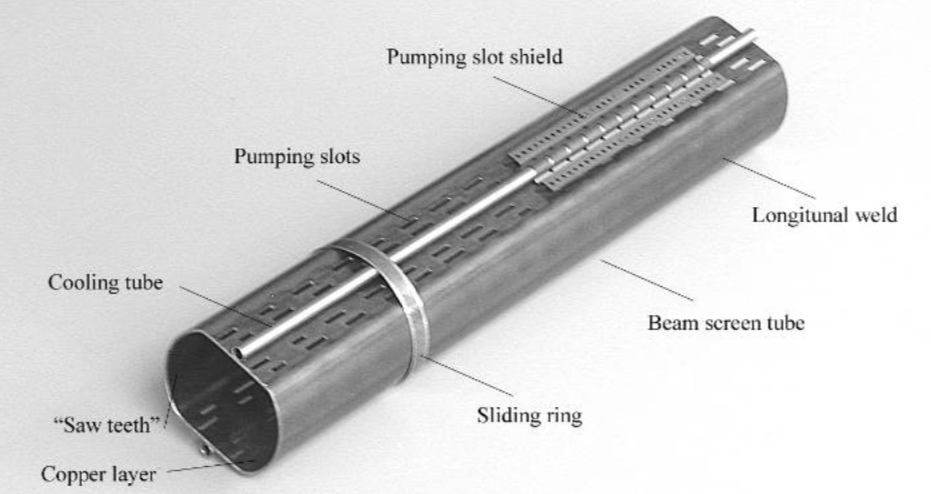
\includegraphics[width=0.7\textwidth]{beam_screen}
  \caption{Beam screen.}\label{beam_screen}
\end{figure}



The beam screens are necessary to reduce the number of protons scattering on the residual gas of the beam pipes, which could lead to a magnet quench and even interrupt the machine operation. The table below summarises the main heat sources that degrade the vacuum quality in the beam pipe, where the vacuum must exist at 1.9 K:


\begin{itemize}
\item synchrotron radiation (0.2 $W/m$ per beam),
\item energy loss by nuclear scattering (30 $mW/m$ per beam),
\item image currents (0.2 $W/m$ per beam),
\item electron cloud related effects (vary).
\end{itemize}



Now, that we discussed the LHC collider, we can continue with one of the main LHC detectors - the CMS detector - the one that was used to collect the data analysed in this thesis. 

%%%%%%%%%%%%%%%%%%%%%%%%%%%%%%%%%%%%%%%%%%
%%%%%%%%%%%%%%%%%%%%%%%%%%%%%%%%%%%%%%%%%%
%%%%%%%%%%%%%%%%%%%%%%%%%%%%%%%%%%%%%%%%%%
%%%%%%%%%%%%%%%%%%%%%%%%%%%%%%%%%%%%%%%%%%
%%%%%%%%%%%%%%%%%%%%%%%%%%%%%%%%%%%%%%%%%%
%%%%%%%%%%%%%%%%%%%%%%%%%%%%%%%%%%%%%%%%%%
%%%%%%%%%%%%%%%%%%%%%%%%%%%%%%%%%%%%%%%%%%
%%%%%%%%%%%%%%%%%%%%%%%%%%%%%%%%%%%%%%%%%%
%%%%%%%%%%%%%%%%%%%%%%%%%%%%%%%%%%%%%%%%%%
%%%%%%%%%%%%%%%%%%%%%%%%%%%%%%%%%%%%%%%%%%
%%%%%%%%%%%%%%%%%%%%%%%%%%%%%%%%%%%%%%%%%%
%%%%%%%%%%%%%%%%%%%%%%%%%%%%%%%%%%%%%%%%%%
%%%%%%%%%%%%%%%%%%%%%%%%%%%%%%%%%%%%%%%%%%
%%%%%%%%%%%%%%%%%%%%%%%%%%%%%%%%%%%%%%%%%%
%%%%%%%%%%%%%%%%%%%%%%%%%%%%%%%%%%%%%%%%%%
%%%%%%%%%%%%%%%%%%%%%%%%%%%%%%%%%%%%%%%%%%
%%%%%%%%%%%%%%%%%%%%%%%%%%%%%%%%%%%%%%%%%%


\section{The CMS experiment}

EGAMMA AT LEAST SAY THAT HAS BEEN WORKING AND SHOW SOME PLOTS???
   
   The logical blocks might include:
  - general comments that the CMS experiment revolves around the CMS deteector which is a general purpose particle deteector placed in a cavern around one of the interaction points at the LHC, and is capable of detecting and measuring properties of particles of all sorts with the exception of neutrinos, etc.
  - requirements that drove design choices for the CMS deteector can be discussed AS A SUMMARY AT THE END???
  - somewhere a section on physics objects where you discuss that there are tracks, there are jets, there are b-jets, what it means an isolated lepton, what it means missing momentum, and so forth. For example, Ekaterina has a section on particle flow, if I remember right, where she discusses that. Or you can have a section that just discuses the proton-proton collisions environment and explains that many particles created in collisions are unstable and decay right away. What is observable in an experiment such as CMS is longer-lived or stable particles. These include electrons, muons, photons, and some ground state hadrons. At the same time, energetic quarks or gluons hadronize and can be seen in a particle detectors as jets of hadrons (so define jets here). Same for tau leptons, we detect them either as electrons/muons, or hadronic jets. Etc. If you have such a conceptual paragraph here, some time later you can have a particle flow discussion when it is time to be more specific. But discussion at this level above would allow you to then discuss the requirements on CMS design using terms like b-jets or isolated leptons.
  - the coordinate system section is good to have.
  - the CMS detector section
  - consider also discussing the trigger system after discussing all subdetectors, this could be part of the CMS detector section.
  
  
%%%%%%%%%%%%%%%%%%%%%%%%%%%%%%%%%%%%%%%%%%%%%%%%%%%%%%%%%%%%%%%%%%%%%%%%%%%%%%%%%%%%%%%%%%%%%%%%%%%%%%%%%%%%%%%%%%%%%%%%%%%%%%
START IS HERE                        

The Compact Muon Solenoid (CMS) is a multi-purpose particle detector built to study a variety of complex particle interactions produced by the LHC. CMS is located in the underground cavern at the "Point 5", which is one of the four main IPs of the LHC. The CMS detector with the additional computing infrastructure is able to detect the produced particles, measure their main physics parameters, and to send the related data to computing data centres for persistent storage. 


The CMS detector has a cylindrical shape and consists of a central ("barrel") and two forward ("endcaps") sections (see Fig. \ref{CMS_detector}). 
CMS is the heaviest detector ever built with the mass of nearly 12500 tons. The mass is explained by the amount of the used superconducting metal, which serves as the magnet. The CMS is 21.6 m long and 14.6 m high. The CMS has an onion-like structure of concentric layer of detectors around the IP. In addition, at the outer part it has a large superconducting solenoid to produce inside the detector a homogeneous magnetic field of 3.8 T. This magnet is the core of the experiment, it is a NbTi superconducting solenoid of 6 m in diameter that operates at a temperature of 4.5K. This magnetic field bends the trajectories of charged particles and is of utmost importance for the CMS. 


\begin{figure}[H]
  \centering
  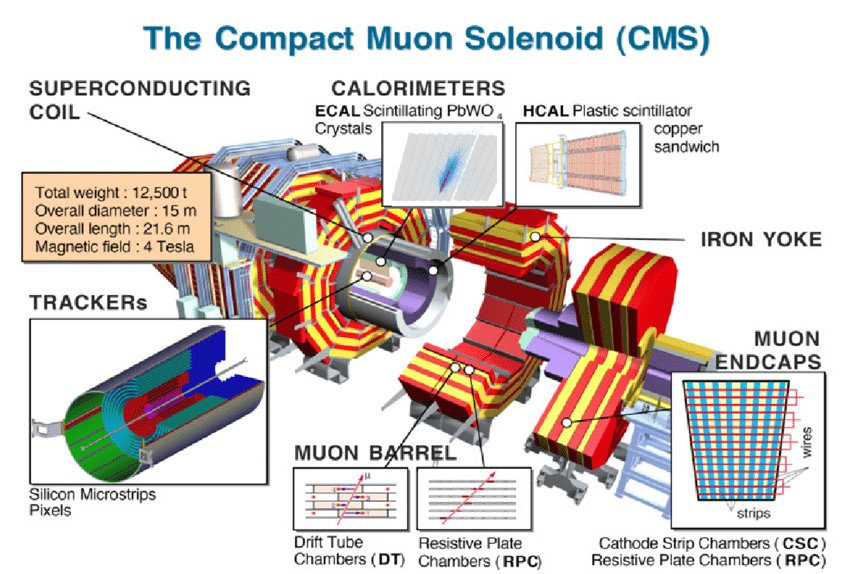
\includegraphics[width=0.8\textwidth]{CMS_detector}\\
  \vspace{1cm}
  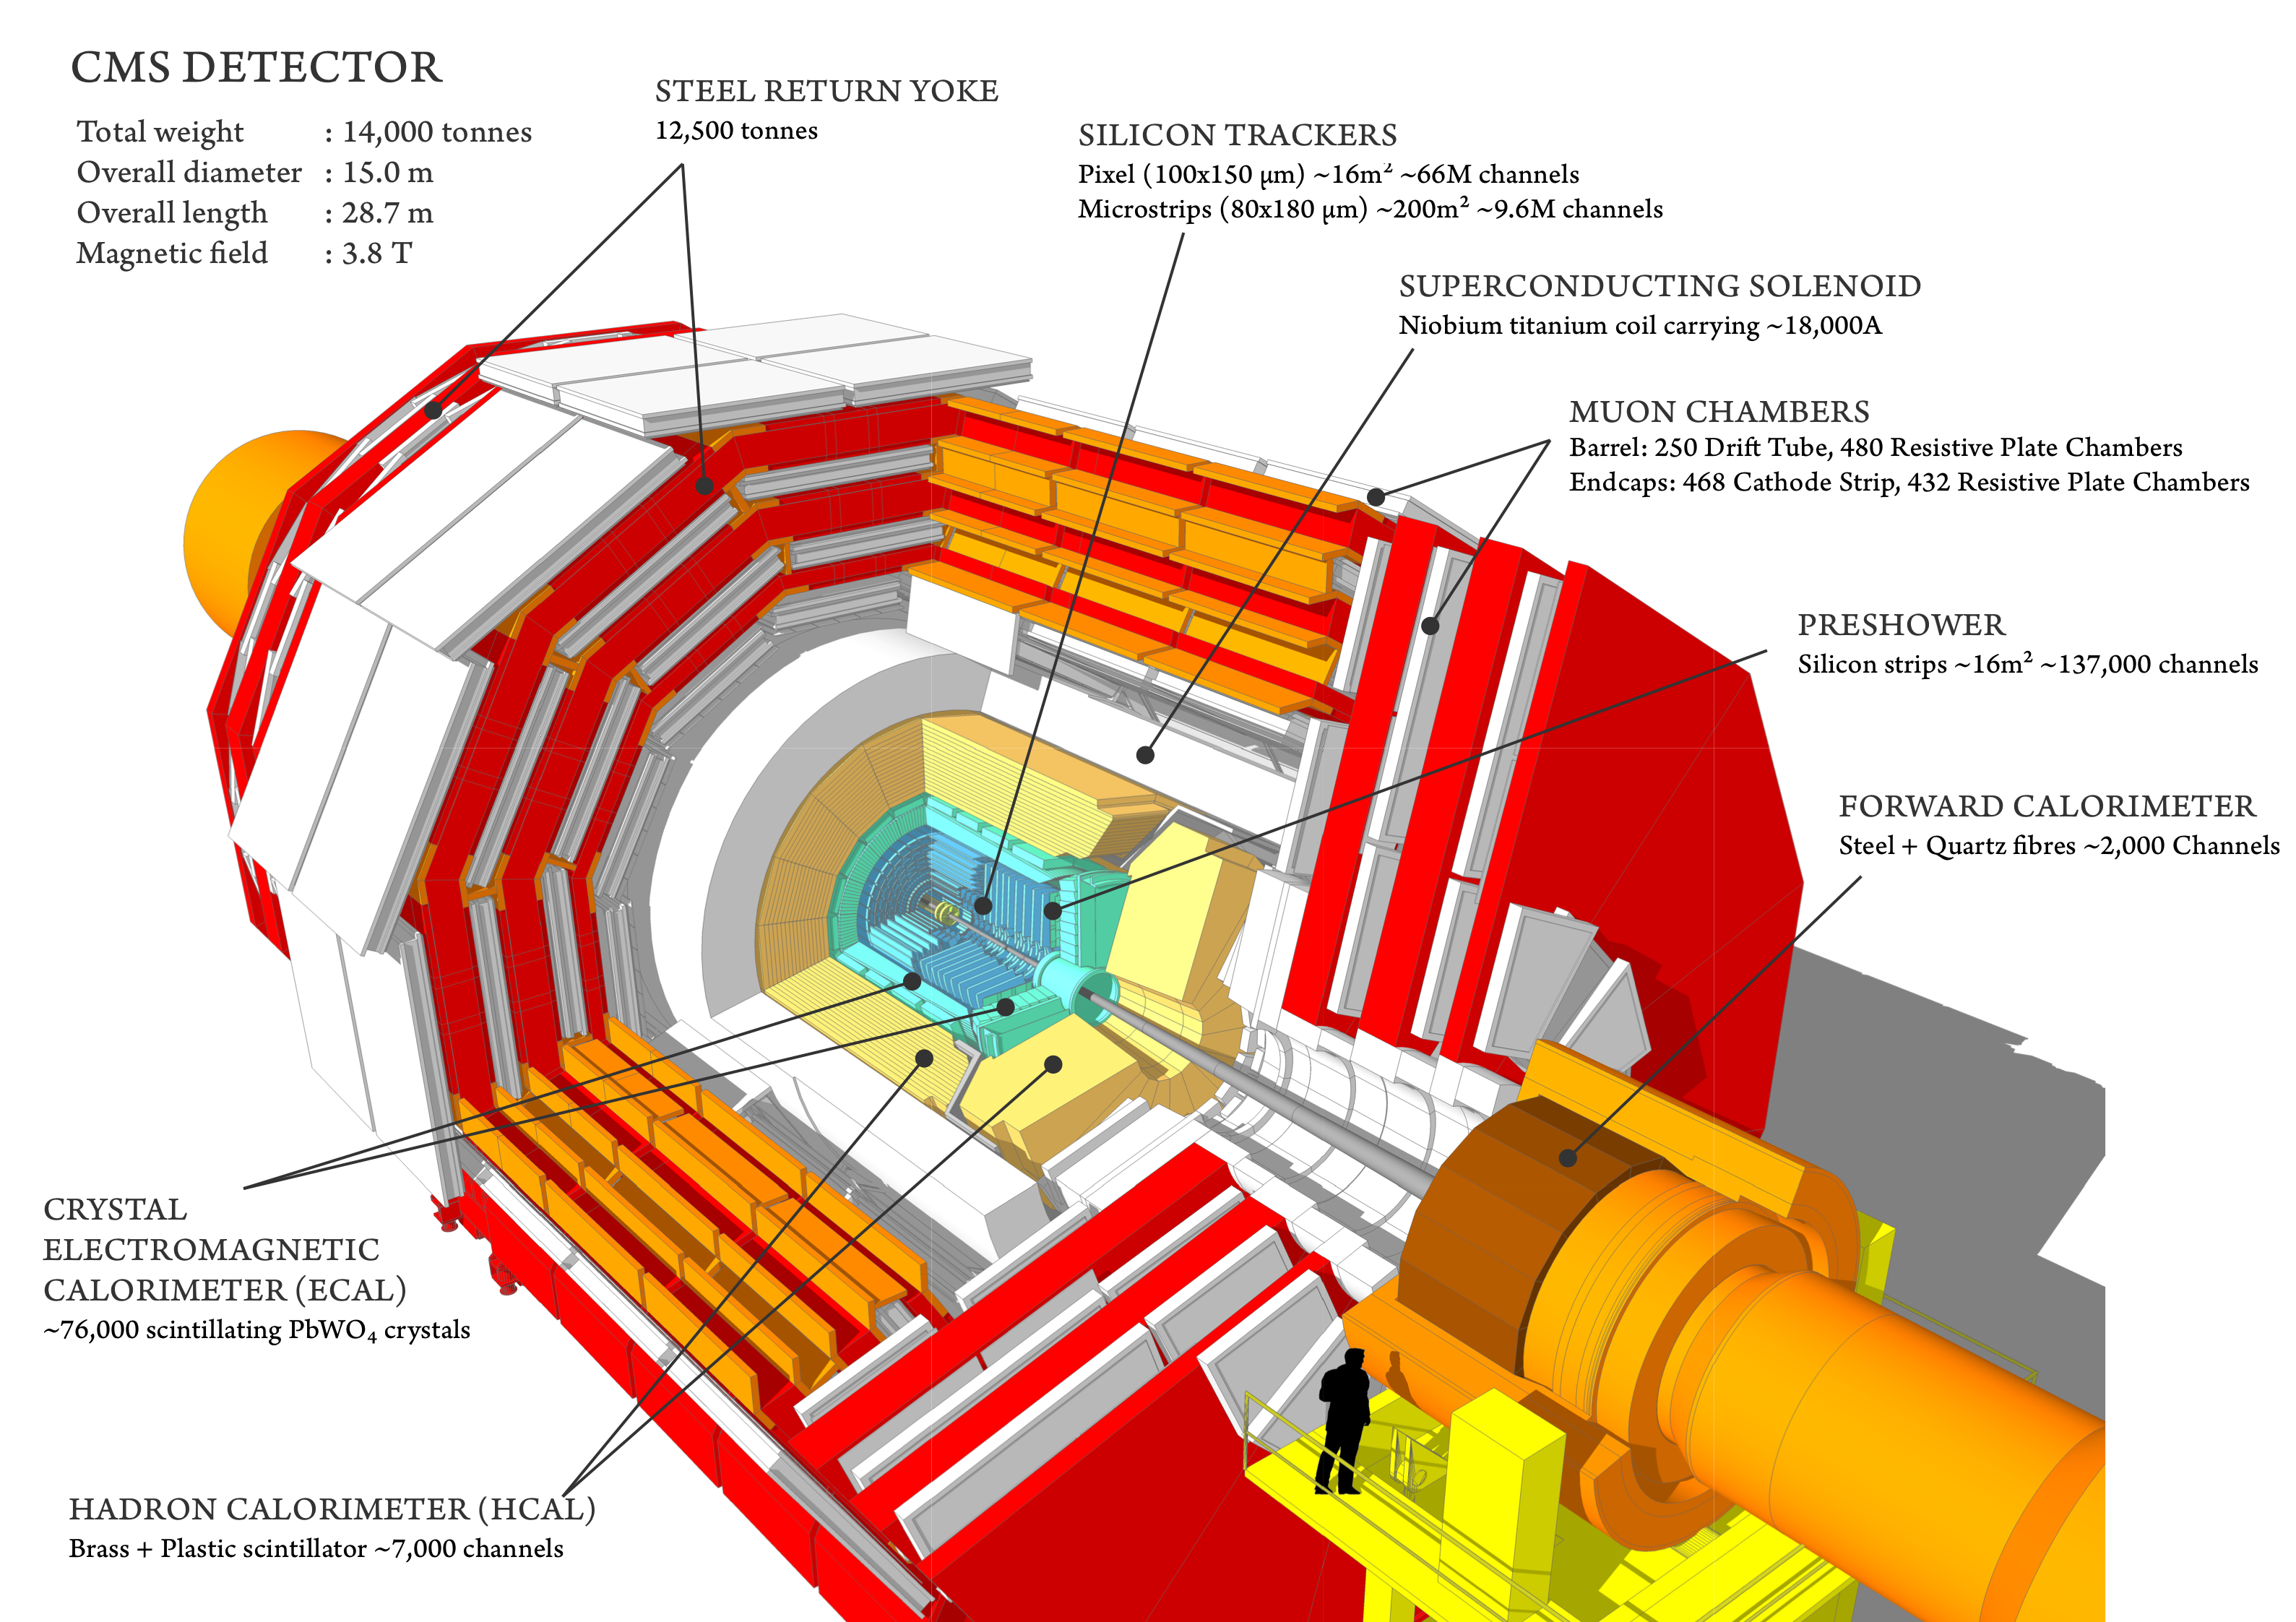
\includegraphics[width=0.8\textwidth]{cms_cross_section}
  \caption{CMS experiment with the main sub-detectors.}
  \label{CMS_detector}
\end{figure}


All sub-detectors can be categorised into trackers and calorimeters \cite{Hauptman:2011zza}. As the particle passes through the material of the tracker, it leaves a "track", which is a path of the emerging particle. Trackers focus on the direction and the track curvature of the charged particles. Tracking information allows the determination of the particle's momentum. 

There are two trackers in CMS: an inner tracking system that encloses the IP and the outer tracking system that is located outside of the solenoid magnet. The first system contains the Pixel and the Strip trackers. The second tracking system is dedicated for the muon detection and is usually called a muon tracker or a muon system. This system is embedded within a steel yoke of the magnet. Such an arrangement saves the CMS some space and also guarantees that the magnetic flux lines are closed. This structure provides a return field of the magnet of about 2 T and is used to measure the momentum of muons. This "two-directional" magnetic field with respect to the magnetic yoke, causes the muons trajectories to be bent in opposite directions in the inner tracker in contrast to the outer tracker. This important feature of the CMS detector is depicted in the CMS logo (see Fig. \ref{cms_logo}). 

\begin{figure}[H]
  \centering
  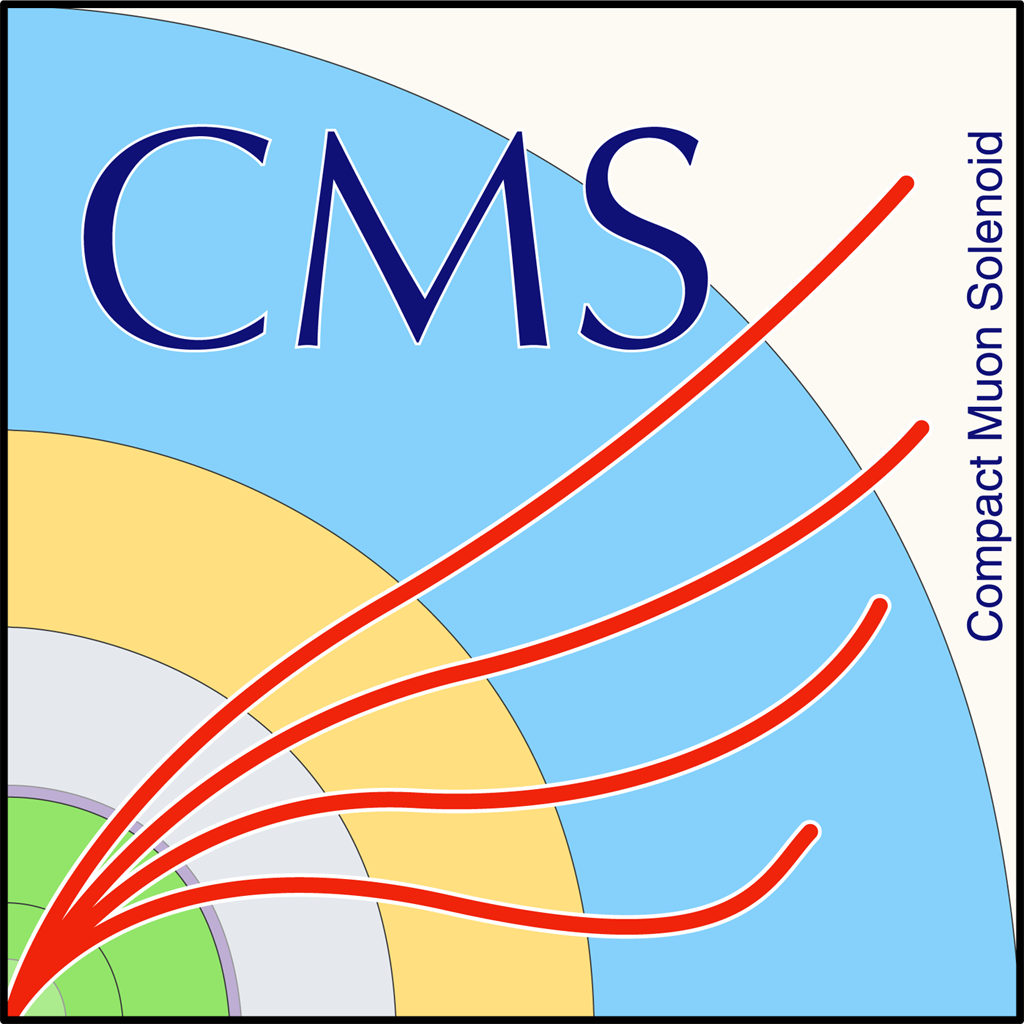
\includegraphics[width=0.4\textwidth]{cms_logo}
  \caption{The logo of the CMS experiment that is showing curved trajectories of the emerging muons.}
  \label{cms_logo}
\end{figure}


The CMS has two calorimeters: the electromagnetic and the hadronic calorimeters. They both rely on high density materials either to sample or to contain almost all the energy of the incoming particles with their secondary interaction products. However, these two systems focus on two different sets of particles. As will be discussed later, electromagnetic calorimeter (ECAL) is dedicated to measuring the energy of photons and electrons, while the hadronic calorimeter is targeting the measurement of the energy of hadrons. %Also, calorimeter information can be used to estimate the direction of the particle. 


Lastly, the rate of the incoming data is 40 MHz. This corresponds to almost 40 TB produced every second. This much data is impossible to store, and, most importantly, most of the information in this data is not interesting for future physics analyses. To reduce the data rate, the CMS uses a highly efficient system of triggers. The first one, the Level-1 (L1) trigger, reduces the nominal collision rate of 40 MHz to 100 kHz. The subsequent High Level Trigger (HLT) further decreases the rate to 1 kHz. With the help of the trigger system, the original 40 TB per second rate is transformed into manageable 1 GB per second that is stored for offline analysis use. 



\subsection{The CMS coordinate system}

A right-handed Cartesian coordinate system is used to describe the detector and the collision products. It is defined with its centre in the nominal interaction point, the x axis pointing to the centre of the LHC ring, the y axis pointing upwards, and the z axis pointing in the anticlockwise proton beam direction.
Given the cylindrical structure of the detector, a polar system is also used. The azimuthal angle ? is defined in the (x, y) or ?transverse? plane as the angle formed with respect to the positive x axis, and the radial coordinate in this plane is denoted as r. The polar angle ? is defined in the (r, z) plane as the angle formed with the z axis and usually converted into the pseudorapidity ? = ln tan(?/2). The spatial separation of two particles can be expressed in terms of their angular distance as (?R)2 = (??)2 + (??)2.
The projection of the momentum of a particle onto the transverse plane is referred to as the ?transverse momentum? or pT, and has the advantage to be independent on the Lorentz boost resulting from the initial momentum of the interacting partons along the z axis.


The information from the individual subdetectors are often redundant and can be combined to improve the reconstruction of final state objects, as it is discussed in Sec- tion 2.3.







We repeat and extend here the conventions given at the beginning of Chap. 1, to clarify their relationship with the geometry of CMS. The coordinate system used by CMS is a right-handed orthonormal system with its origin at the nominal IP, its x-axis directed toward the centre of the LHC ring, its y-axis pointing vertically upwards, and its z-axis thus being tangent to the counter-clockwise (when viewed from the top) circulating beam trajectory, pointing away from Lake Geneva. These define in turn the azimuthal










angle ?, measured from the x axis in the x-y-plane (transverse plane), and the polar
??
The transverse momentum pT is computed as the magnitude of the projection of the measured momentum p????(px,py,pz) in the transverse plane; the ?transverse energy? of a particle with energy E is given by ET ?? sin ? � E. In the following, the direction of particles produced at the IP will be quoted as a function of ? and the pseudorapidity:


 22 x + y .
? ?? ? ln tan ?/2 (2.5.)
For massless particles, this quantity is equal to the rapidity y. From this point on, angular distances are defined using the pseudorapidity, i.e.:
??
22
?R?? (?1??2) +(??) ,with (2.6.)
????min??|?1??2|,2??|?1??2|??. (2.7.)
The subdetectors composing CMS, as well as the trigger and data acquisition systems, are briefly described in the following sections. More information about the CMS detector can be found in Ref. [170].



%%%%%%%%%%%%%%%%%%%%%%%%%%%%%%%%%%%%%%%%%%%%%%%%%%%%%%%%%%%%%%%%%%%%%%%%%%%%%%%%%%%%%%%%%%%%%%%%%%%%%%%%%%%%%%%%%%%%%%%%%%%%%%


  
  
The total inelastic cross section of the proton-proton interaction at $\sqrt{s}=13$ is about 70 $m$b. The detectors observe the event rate of nearly $10^{9}$ inelastic events per second.


  In addition, a pile up DEFINE (PU) of 20-200 events overlaid with the event of interest will be expected, 
  
  which results in about 1000 particles produced every 25 ns. 
  
  INTRO ALL SUBDETECTORS
  
  
  
  
  All sub-detectors of CMS (see Fig. \ref{CMS_detector}), thus, have to be able to work fast and in a good synchronisation with each other. 




3. What you want to convey, perhaps, is that to achieve its physics goals, or successfully complete its physics program, or such, the CMS detector is designed to have: good momentum resolution, etc etc, or the design goals for the CMS detector required for success of the CMS phusics program were?


One can summarise all challenges and requirements that the CMS has faced in the following list:

You mention throughout this bullet list CMS systems: tracker, ECAL, HCAL, and what requirements are imposed on their design. But the reader at this point has no idea what these systems are.

Generally, a lot of stuff is undefined here and in the above bullets. Maybe every single thing would be painful to  define, but a non-collider physicist will be lost quicjly here. 
  What is diphoton, dijet mass? 
  What is ?missing transverse mass??
  What is a jet? What is a b-jet?
   What are isolated leptons and photons?
  You are thrusting a reader into a jargon-rich environment without preparation.


\begin{itemize}
\item good muon momentum resolution over the momentum scale covering almost a TeV range, good dimuon ??????resolution at the 100?????/ GeV, and a capability to determine correctly the charge of the highly energetic muon all the way up to 1 TeV
\item good momentum resolution of the charged particles in the inner tracker. CONNECTION Emphasis on the efficient $\tau$ lepton and b-jets reconstruction
\item good performance of the electromagnetic calorimeter (ECAL), with the particular attention to the diphoton mass resolution, ability to reject efficiently $\pi^0$ EXPLAIN, ability to identify isolated photons and leptons
\item good missing transverse mass and dijet-mass resolution, which depends heavily on the performance of the hadronic calorimeter (HCAL)
\end{itemize}

The first part, the bullet list of the design goals, seems not connected in any way to the detector description that follows. Not even clear to me why these two are in the same section.


The CMS design has been driven by the needs to have a large bending power, which is to be provided by the superconducting magnet, to be able to disentangle ............??????/various charged particles. 

The paragragh structure is odd: you have one paragraph discussing the magnet + strip tracker, and a separate paragraph is fully devoted to pixels. Odd grouping.






The size of the magnet is 13 m in length and 6 m in inner diameter. 4 T solenoid provides 12 Tm bending power. The inner  DEFINE diameter is large enough to host the inner tracker and the ECAL. To address the high multiplicity problem???, the CMS inner tracker uses 10 layers of the silicon microstrip detectors. The inner barrel contains four layers of strips and the outer barrel has six layers. Each silicon sensor is 320 $\mu m$ in height and a specifically designed overlay of strips provides a spatial resolution of 13-38 $\mu m$. About the same resolution is achieved by the other tracker. The whole tracker contains 15148 silicon modules with the 9.3 million strips. Tracker provides the experiments with the tracks information left by the charged particles traversing its material. 

To further improve the impact parameter determination and secondary vertex reconstruction, three layers of the silicon pixel detector are inserted near the interaction region. Pixel detector ADD DETAILS OR REMOVE SOME FROM THE INNTER TRACKER is composed of 1440 silicon pixel detector modules organised in three concentric cylindrical layers, and also two disks in the forward regions. 


PURPOSE OF ECAL The ECAL technology is based on the on the lead tungstate crystals ($PbWO_4$). The ECAL measures the energy deposited by photons and electrons. ECAL contains 75848 crystals where the energy showers???? will be produced by the particles releasing their energy when interacting with the material of the crystals. Before the ECAL, a preshower system is placed to reject $\pi^0$. 

1. How does the preshower system ?reject? pi0?  Actually, data from the preshower subdetector allow us to identify pi0 (and thus reject pi0 candidates in the measurements where they are a background).
2. The preshower subdetector is there only in the endcap, by the way.


It contains layers of lead radiators followed by layers of the silicon strips to initiate???? and subsequently to measure the energy of the particle. The ECAL measured energy of the particles is a function of the stochastic term (S), noise (N), and a constant term (C). 

It is not a function of the stochastic term, etc. It is a function of energy, and the expression contains the stochastic term, the noise term, etc.
  Also, have the ?:? at the end, and ?.? at the end of the equation.
  
  
\begin{equation}
  \left(\frac{\sigma}{E}\right)^2 = \left(\frac{S}{\sqrt{E}}\right)^2 +
  \left(\frac{N}{E}\right)^2 + C^2
  \label{eq:ecal}
\end{equation}

The ECAL 
magnet
then
HCAL system

 which is based on the brass/scintillator sampling hadronic technology. HCAL measures energy of particles made of quarks. 
 
 What does it mean ?later?? Later usually refers to time sequence.

Why is tail-catcher italicized, are you consistently using this method to introduce new terms? But you do not explain this term here. (You had plenty of unknown terms before, like kickers or tracker, and never italicized those).
   Also, in general, I do not understand this sentence, what does it mean ?leaving 11 hadronic interactions?, how ?11? is to be interpreted (a lot? little?), etc.
   
   
   Central part is later covered by the $\textit{tail-catcher}$ leaving 11 hadronic interaction lengths to the particle interactions.  
Further, the forward calorimeter is used to ensure the coverage in $\eta$ up to 5. Note, that the coverage of ECAL and HCAL are about up to $\eta=3$.  

Is this forward calorimeter part of HCAL or not? If it is, then the next sentence seems to contradict this eta=5. If it is a different subdetector, I do not know whether to expect that it uses the same technology, has the same reoslution, uses the same principles, or not.


If you want to list the eta coverage of different subdetectors, then list this in the right place (e.g. HCAL measures energy of hadrons with the eta range ? ? etc.), not tucked in at the end as an afterthought.




Additional dedicated detectors such as  CASTOR, ZDC, etc, ensure that the detector has almost a full $4\pi$ coverage. 

The paragraph content seems unbalaanced. HEre you switch to other detectors, and then you come back to the HCAL.

HCAL does not fully absorb energy of the the particles traversing its medium, except very low energy particles, thus the energy of the particles is sampled to estimate the total amount.  

I am missing something her. The HCAL contains vast majority of showers initiated by hadrons in full. Because it has 11 radiation lengths in depth. Which is because it was designed as a sampling calorimeter, with a lot of absorber. Why do you say that HCAL only fully absorbs energy for vey low energy particles? This doesn?t make sense.
   Also, energy of the particles is sampled is very unclear. In fact, what is sampled is the energy of the shower developing through HCAL that was initiated by the original paricle we wnt to measure. Outer HCAL is located outside of the magnet.

   
   
   
Overall, the CMS detector is 21.6 m in length and 14.6 m in diameter. The weight of the whole construction is near 12 500 tons. ECAL covers more than 25 radiation lengths, HCAL, from 7 to 11, depending on the $\eta$ region. 
It is not clear that that?s the best way to summarize, listing ECAL and HCAL radiation lengths (it is also not trivial presentation, because the reader may not know that ECAL has 25 radiation lengths for photons and electrons, but very little radiation lengths with respect to hadrons).


The superconducting magnet of CMS provides the experiment?????/ make smooth..........??????? is operated at the 4.7 K temperature. 



This discussion of the muon system needs to be improved and made uniform with the discussion of other subdetectors in structure and content. As it is, it reads as an assorted set of sentences, unconnected.
  Also, notice that in some cases you ovewhelm the reader with numbers (like the numbers of crystals or strip sizes,) and in others you hardly mention any numbers of that sort (HCAL, muons).
  
  
  , a magnet yoke is made of five barrel wheels is used for the magnetic flux return and serves as a support for the embedded muon system, which is located outside of the ECAL and HCAL systems. Muons are energetic enough to traverse the ECAL and leave the detector. Tracks in the muon system will be used to reconstruct standalone muons, and in combination with the tracker, to reconstruct the global muons.  


\subsection{CMS coordinate system}

In this section we introduce the coordinate system used in CMS?. You di not need to say that you will use rapidity and pseudorapidity in te analysis section. But you do need to define the directions of the origin of the coordinate system and the directions of the X, Y, and Z.

We will use rapidity and pseudorapidity many times in the analysis section of the thesis. The coordinate system employed by the CMS uses the rapidity, y, and pseudorapidity, $\eta$. They are derivatives of the log functions of the energy and a projection of the momentum of the beam/?????? on the z axis and the angle $\theta$ with respect to the beam axis (see Fig. \ref{coord} \ref{MonroyMontanez:2639240}):


ON THE PIC explain what are eta1, eta2, phi1 and phi2? or FIND A NEW PIC


\beqn
y=\frac{1}{2}ln\frac{E+p_z}{E-p_z} \qquad \eta=-ln \left(tan\frac{\theta}{2}\right)
\label{eqn:eta}
\eeqn


\begin{figure}[h!]
  \centering
  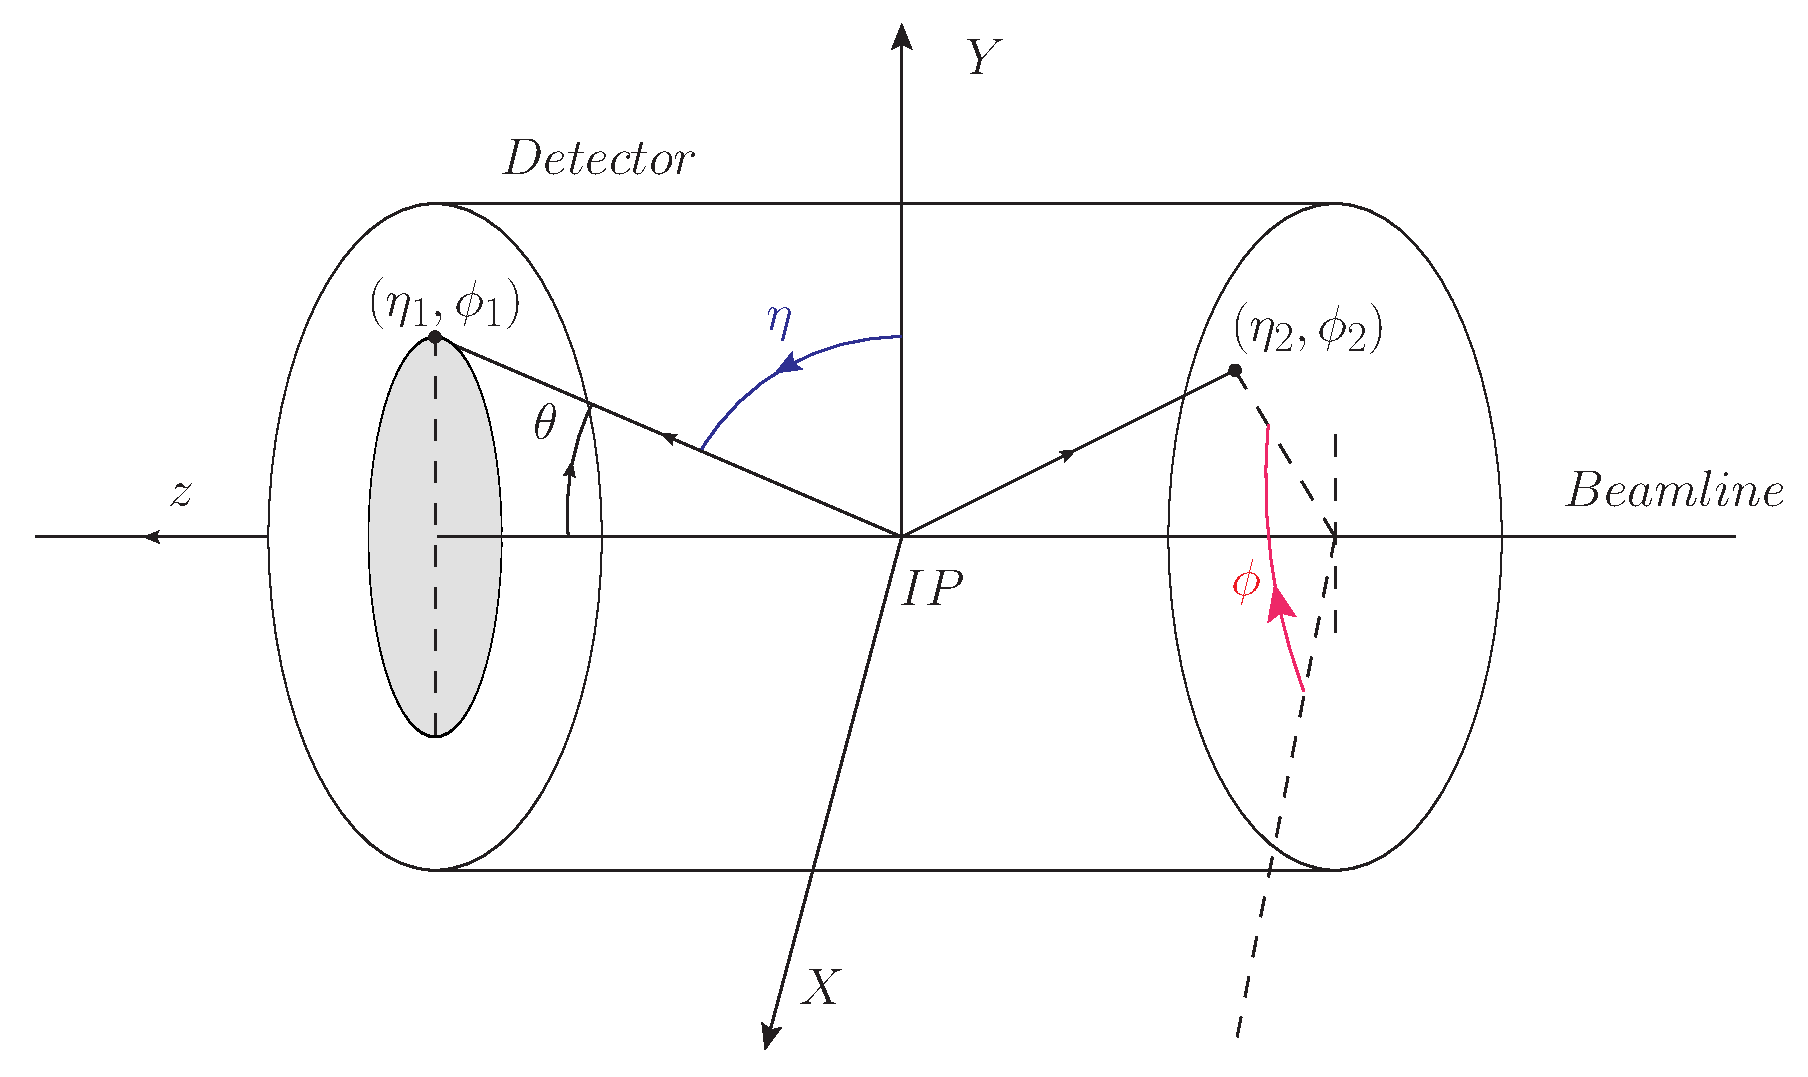
\includegraphics[scale=0.4]{coord}
  \caption[Coordinate system of the CMS detector]{Coordinate system of the CMS detector.}
  \label{coord}
\end{figure}

